\section{Safety Assessment Process}
\label{sec:process}
%\mike{COMPLETELY STOLEN FROM THE SAFECOMP-05 PAPER!  Either note it or modify it}
%\danielle{I added a citation. I think this late in the game we might as well just cite it.}

The overall safety assessment process that is followed in practice
in the avionics industry is described in the SAE standard ARP
4761~\cite{SAE:ARP4761}. This section is a summarization of portions of the ARP 47-61 document (also found in~\cite{Joshi05:SafeComp}). 

\iffalse

This section describes the overall safety assessment process that is followed in
practice in the avionics industry along the lines of the SAE standard ARP 47-61 \cite{SAE:ARP4761}. The descriptions of the various phases of the safety assessment process
covered in this section are essentially based on the ARP 47-61 document.

\fi


\begin{figure}
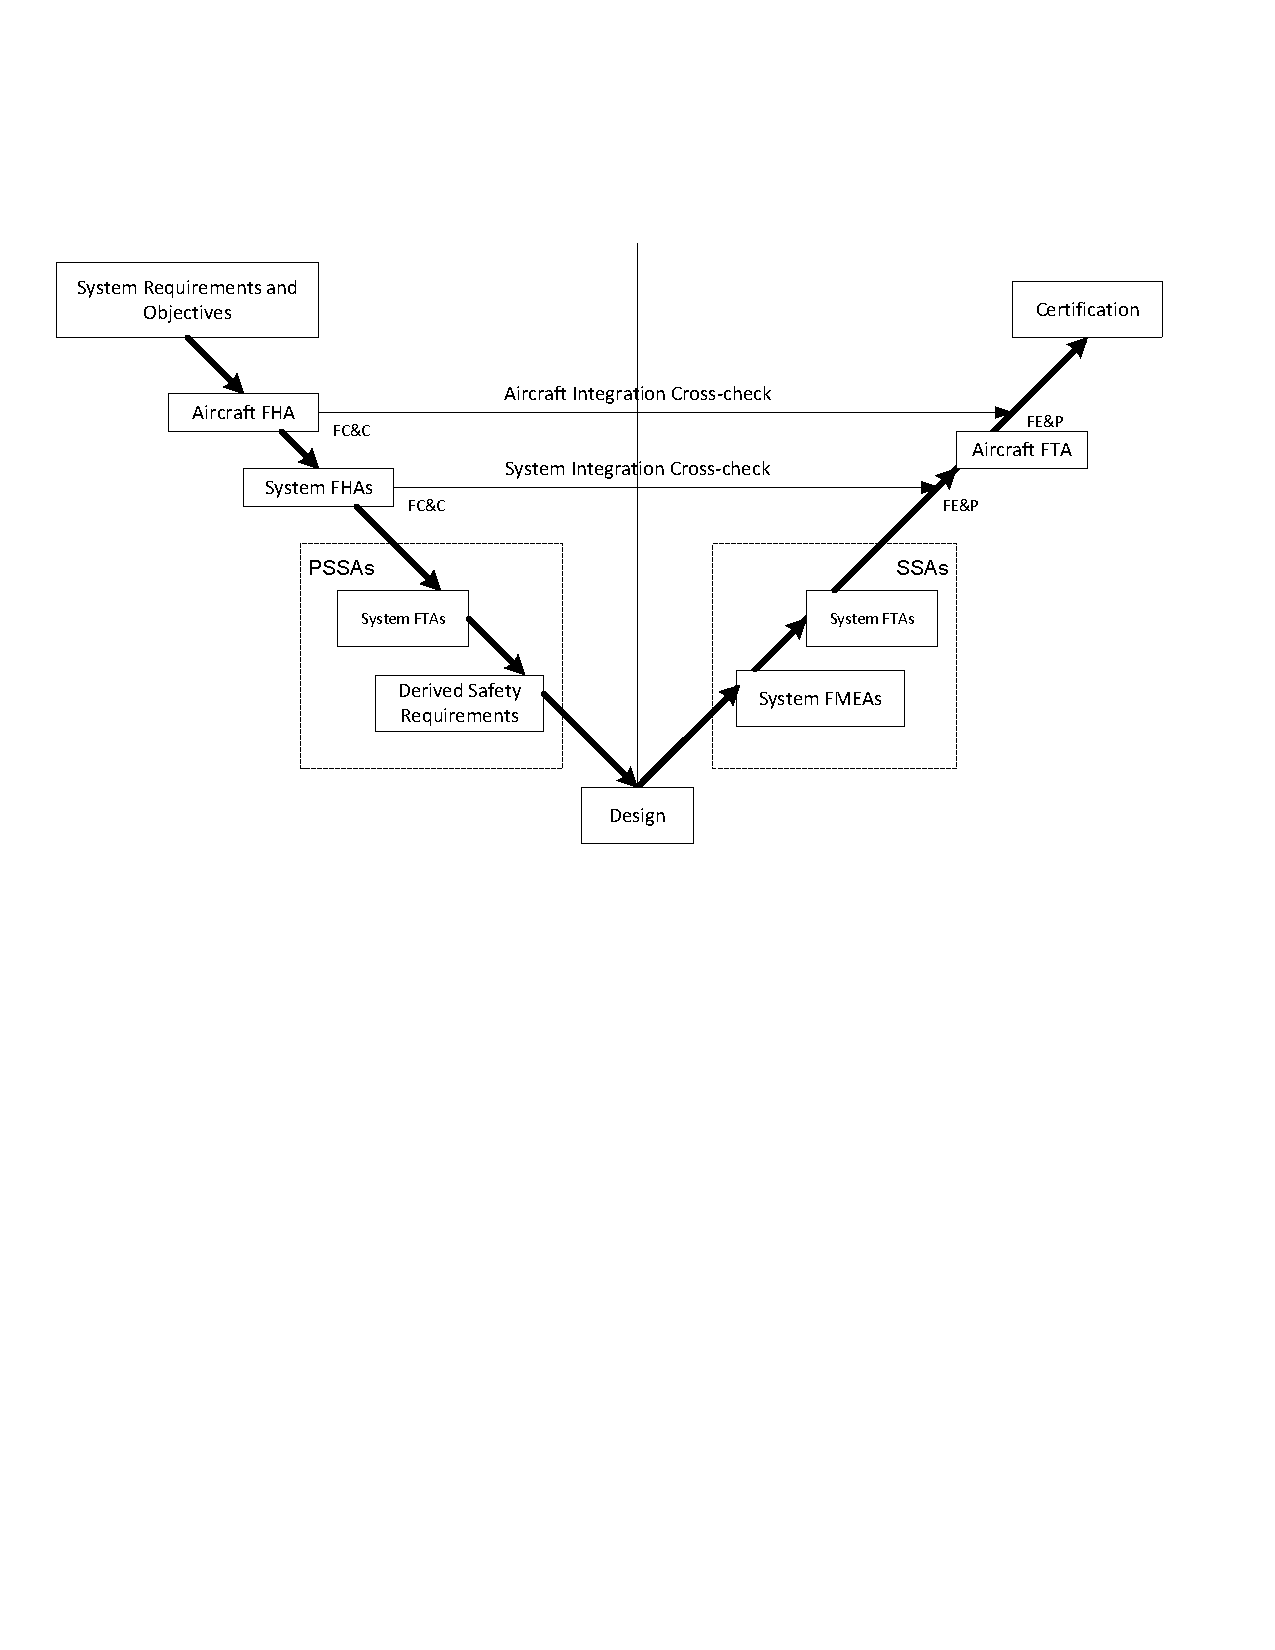
\includegraphics[trim=25 375 0 125, clip, scale=.60]{V}
\caption{Traditional ``V'' Safety Assessment Process} \label{fig:V}
\end{figure}

%The safety assessment process is an integral part of the development process.

Figure~\ref{fig:V} shows an overview of the safety assessment
process as recommended in ARP 4761. The process includes safety
requirements identification (the left side of the ``V'' diagram)
and verification (the right side of the ``V'' diagram), that
support the aircraft development activities. An aircraft level
Functional Hazard Analysis (FHA) is conducted at the beginning of
the aircraft development cycle, which is then followed by system
level FHA for individual sub-systems. The FHA is followed by
Preliminary System Safety Assessment (PSSA), which derives safety
requirements for the subsystems, primarily using Fault Tree
Analysis (FTA). The PSSA process iterates with the design
evolution, with design changes necessitating changes to the
derived system requirements (and also to the fault trees) and
potential safety problems identified through the PSSA leading to
design changes. Once design and implementation are completed, the
System Safety Assessment (SSA) process verifies whether the safety
requirements are met in the implemented design. The system Failure
Modes and Effects Analysis (FMEA) is performed to compute the
actual failure probabilities on the items. The verification is
then completed through quantitative and qualitative analysis of
the fault trees created for the implemented design, first for the
subsystems and then for the integrated aircraft.

%\medskip

We propose to modify this traditional ``V'' process so that the
lower level PSSA and SSA activities are performed based on a
formal model of the system under consideration.
Figure~\ref{fig:Vmod} shows the modified ``V'' diagram for
model-based safety analysis. The shaded blocks are those
activities that will be modified or added.

\begin{figure}
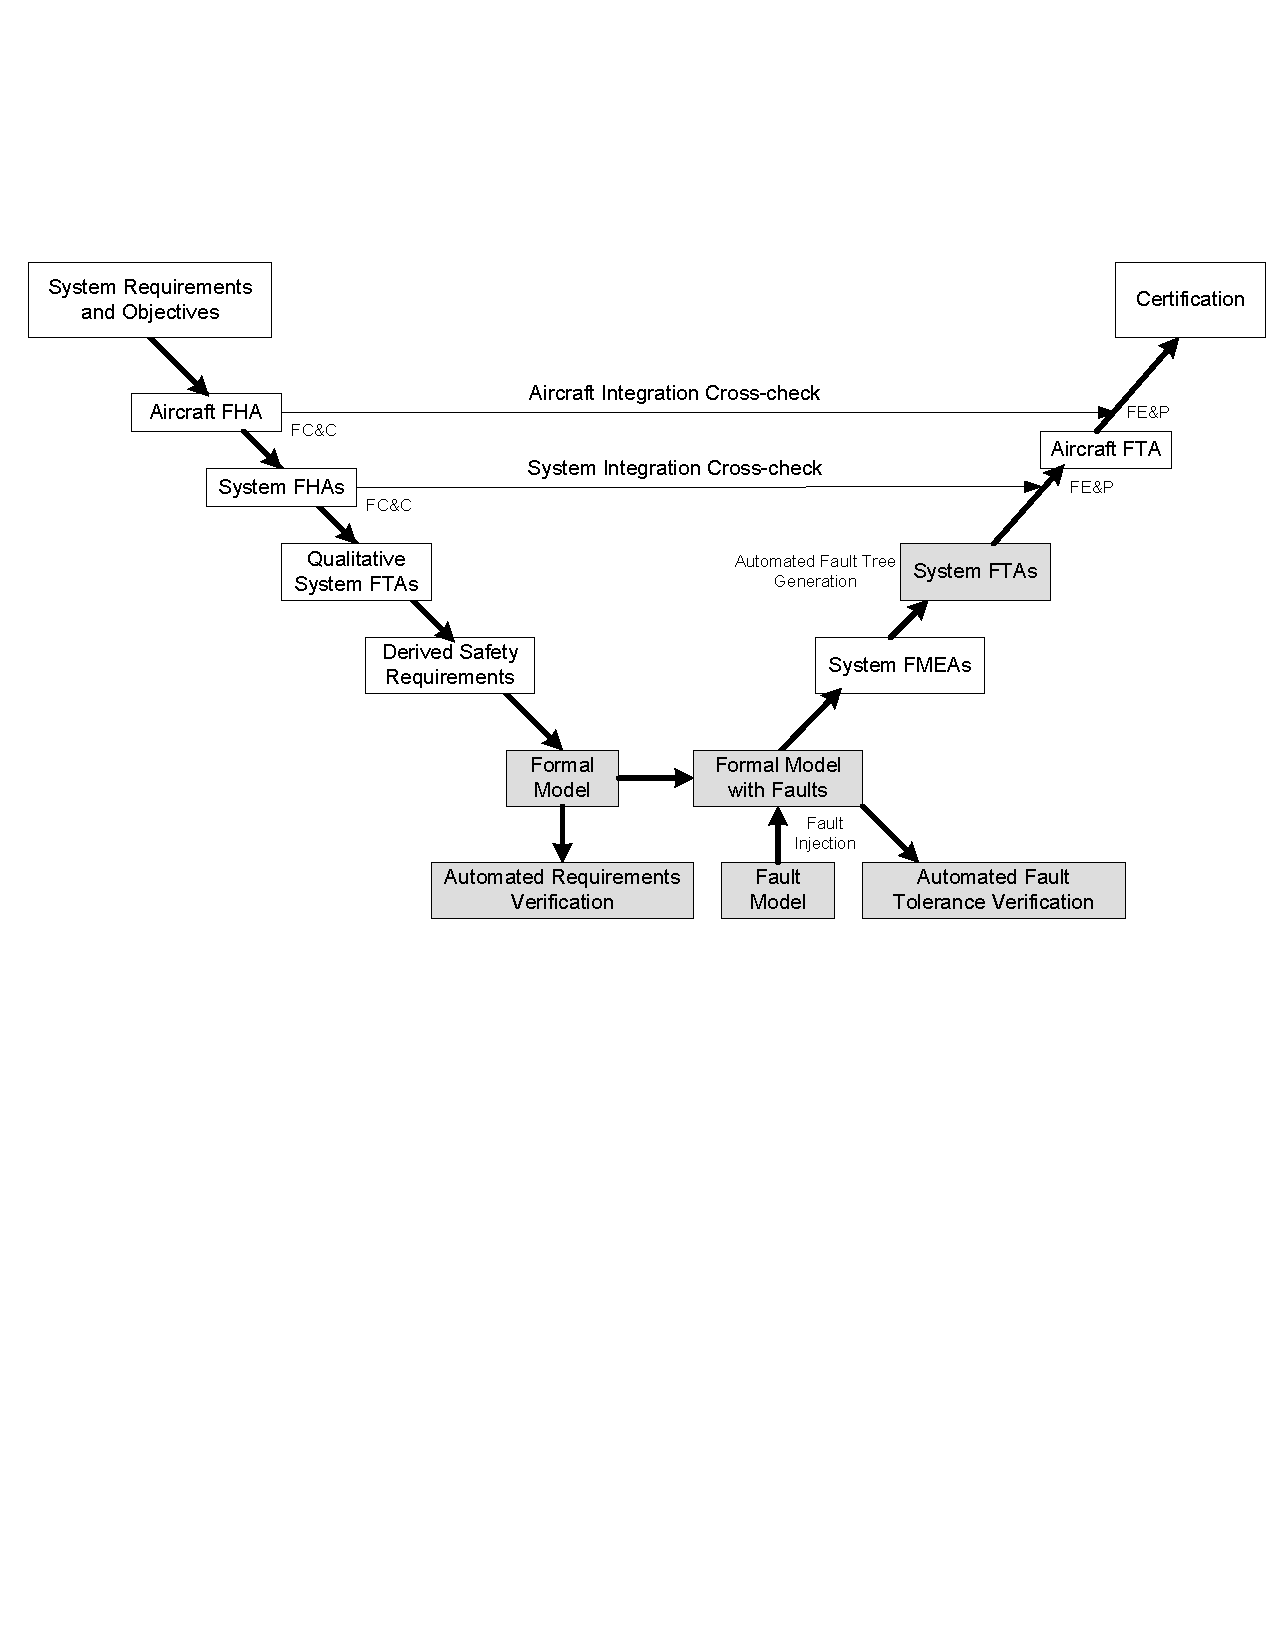
\includegraphics[trim=15 350 0 125, clip, scale=.60]{Mod_V_Process_FaultModel}
\caption{Modified ``V'' Safety Assessment Process} \label{fig:Vmod}
\end{figure}


As we can observe from Figure~\ref{fig:Vmod}, the parts of the analysis that are
primarily affected are at the bottom of the ``V''. The biggest difference is that
the safety analysis activities at this level are now focused around a formal
model of the system behavior, and that many of the artifacts of the safety
analysis can be derived from this model. The idea is to try to pose the right
verification questions to formal tools (such as model checkers and theorem
provers) so that it is possible to derive the necessary safety analysis
information. We then wish to turn the results of these analyses back into
artifacts that can be easily understood and used by safety engineers.
